\chapter{Analiza Dziedziny}
\label{cha:anDziedziny}
%---------------------------------------------------------------------------

\section{Klasy i opis atrybutów}
\label{sec:klasyAtrybuty}
\begin{table}[H]
	\begin{tabular}{|l|l|l|} \hline
	\textbf{Klasa}	& \textbf{Atrybut} & \textbf{Opis} \\ \hline% \bottomrule
	Pojazd	& NumerRejestracyjny & Numer rejestracyjny pojazdu \\ \hline
	Samochód& & \\ \hline
	Motor& &  \\ \hline
	Autobus& & \\ \hline
	Parking	& WolneMiejscaZwykłe & Określa ilość wolnych miejsc dla samochodów na parkingu \\
	& WolneMiejscaAutobusowe & Określa ilość wolnych miejsc dla autobusów na parkingu \\ \hline
	PostójNaParkingu & DataWjazdu & Data wjazdu na parking\\
	& CzasWjazdu & Czas wjazdu na parking \\
	& DataWyjazdu & Data wyjazdu z parkingu\\
	& CzasWyjazdu & Czas wyjazdu z parkingu \\
	& Pojazd & Określa pojazd, którego dotyczy wjazd \\ \hline
	Operator& Id & Id operatora \\
	& Imię & Imię operatora \\
	& Nazwisko & Nazwisko operatora \\ \hline
	Zdjęcie& &  \\ \hline
	\end{tabular}
\end{table}


%---------------------------------------------------------------------------

\section{Diagramy klas  - relacje}
\label{sec:diagKlas}
% Diagram klas
\begin{figure}[H]
	\centering
	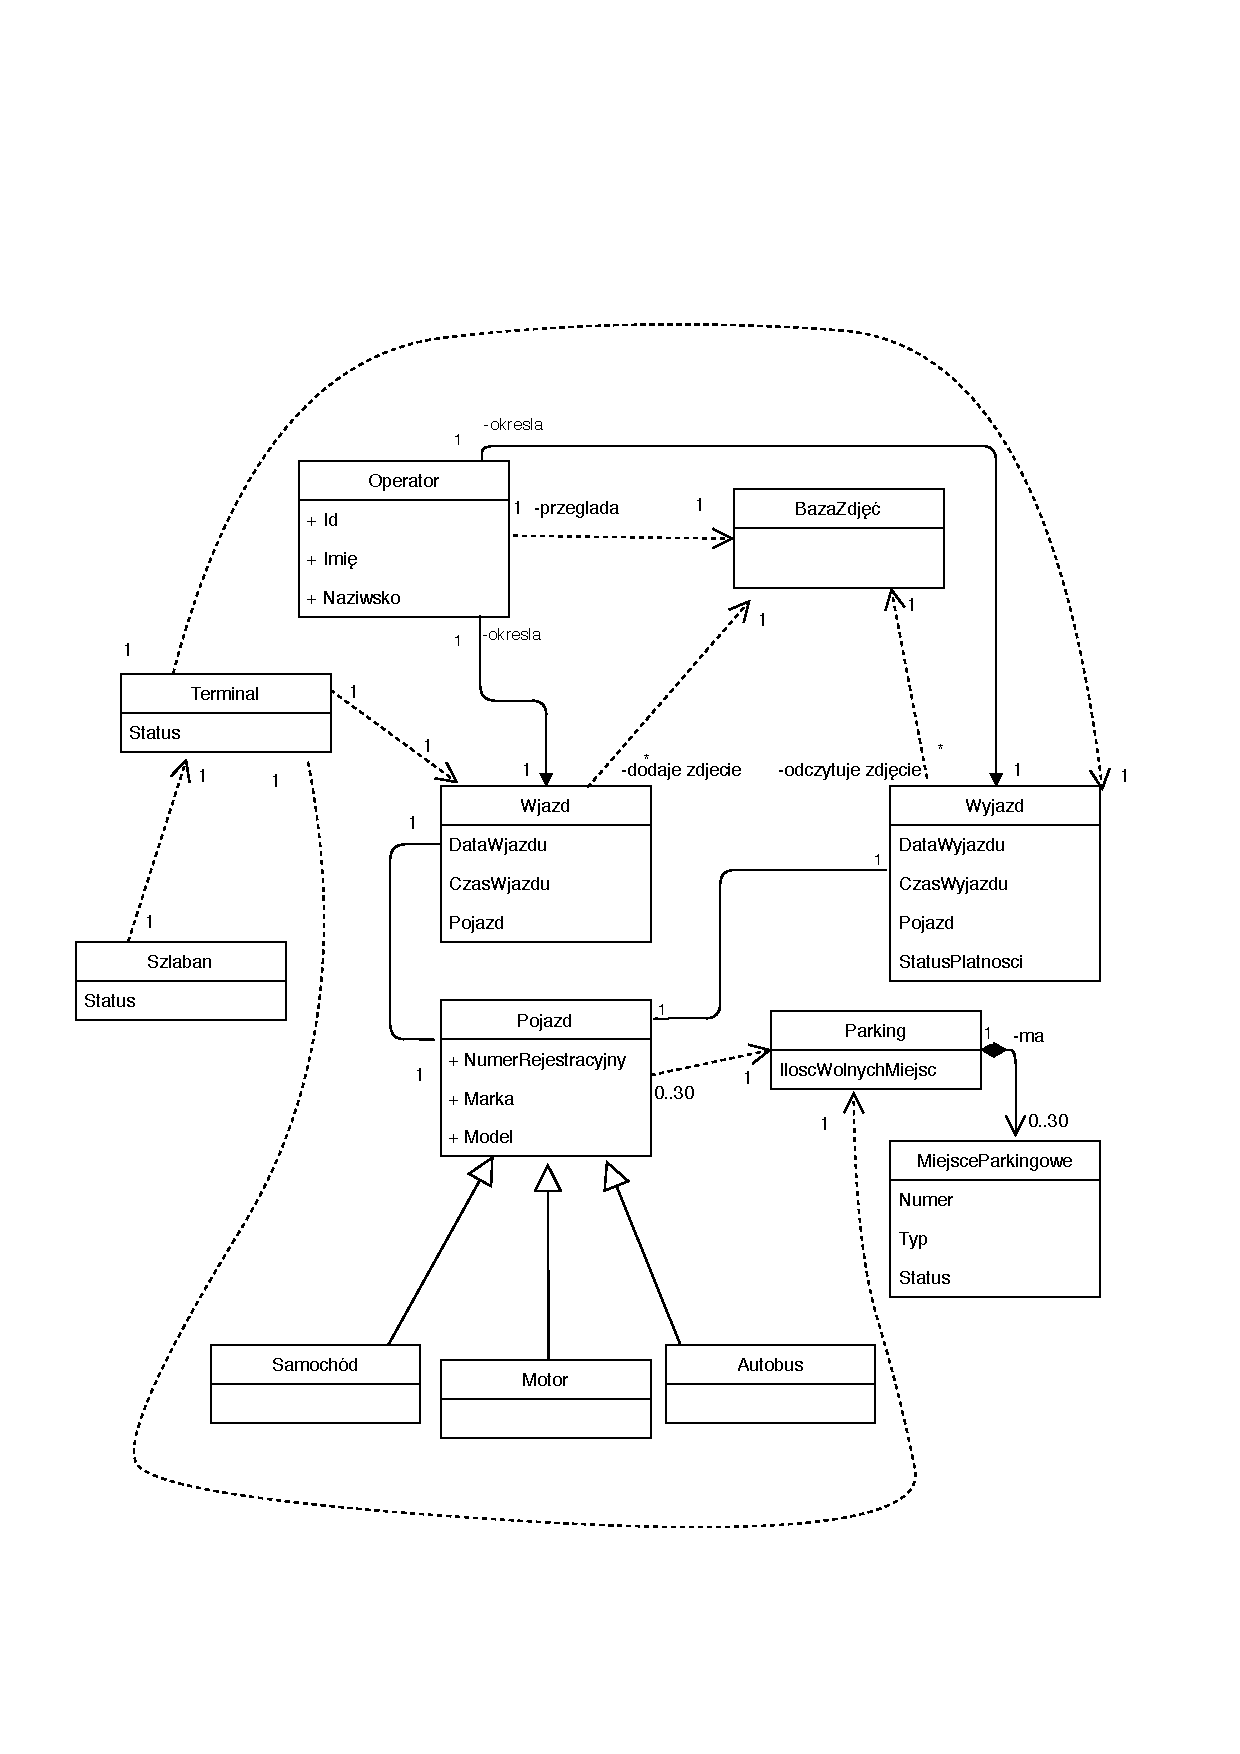
\includegraphics[width=150mm]{diagramy/DiagKlas.pdf}
	\caption{Diagram klas i relacje między nimi}
\end{figure}


%---------------------------------------------------------------------------

\section{Diagramy stanów dla wybranych klas}
\label{sec:diagStanow}
% Diagram stanow
\begin{figure}[H]
	\centering
	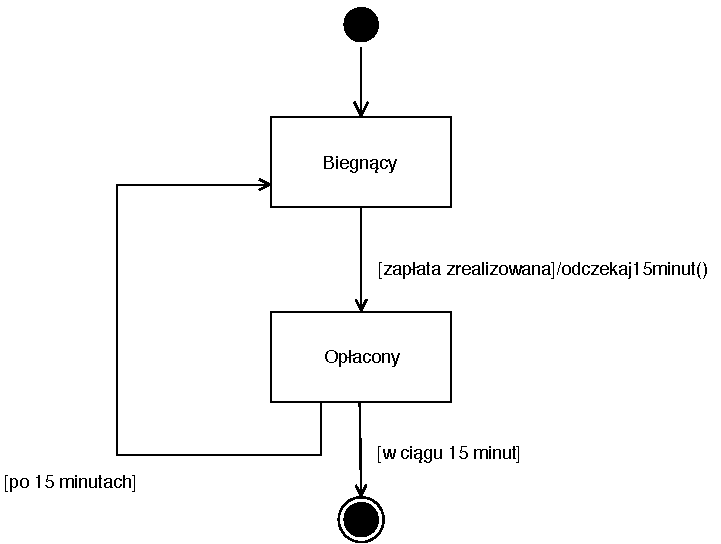
\includegraphics[width=130mm]{diagramy/DiagStanow.pdf}
	\caption{Diagram stanów dla klasy PostójNaParkingu}
\end{figure}



%---------------------------------------------------------------------------

\section{Słownik pojęć}
\label{sec:slownik}

\begin{list}{$\bullet$}{}
\item Klient - wprowadza rejestracje do systemu, potwierdza zdjęcie oraz dokonuje płatności w systemie
\item Operator - pracownik parkingu, identyfikowany na podstawie Id, ma możliwość przeglądania i wyboru zdjęć w przypadku błędu w systemie oraz poprawy rejestracji
\item Parking - przechowuje informacje dotyczące ilości wolnych miejsc (zwykłych lub autobusowych)
\item Pojazd - należy do klienta, na podstawie rejestracji pojazdu jest on wpuszczany i~wypuszczany z~parkingu
\item PostójNaParkingu - klasa reprezentująca postój pojazdu na parkingu wraz z wjazdem i wyjazdem
\item System - służy do obsługi automatycznego parkingu, oblicza płatności, zgłasza błędy odczytu zdjęcia lub rejestracji, a także zbiera dane statystyczne
\item System przetwarzający obraz - zewnętrzny system, robi zdjęcia, przetwarza je oraz zwraca rejestracje naszego systemu
\item Szlaban - może być otwarty lub zamknięty, jego status ustalany jest przez system
\item Terminal - kieruje szlabanem, zbiera informacje o~ilości wolnych miejsc na parkingu, pośredniczy w przetwarzaniu płatności
\item Właściciel - ma możliwość przeglądania statystyk po wcześniejszym zalogowaniu się do systemu
\item Zdjęcie - zdjęcie tablicy rejestracyjnej pojazdu znajdującego się na parkingu
\end{list}
